\section{Tasks}
In this section, research works about five  popular community detection tasks are summarized. The five selected tasks are independent with each other and tackle community detection problems from various perspectives. 

\subsection{Overlapping Community Detection}
\begin{figure}
	% \setlength{\belowcaptionskip}{-10pt}
	\center
	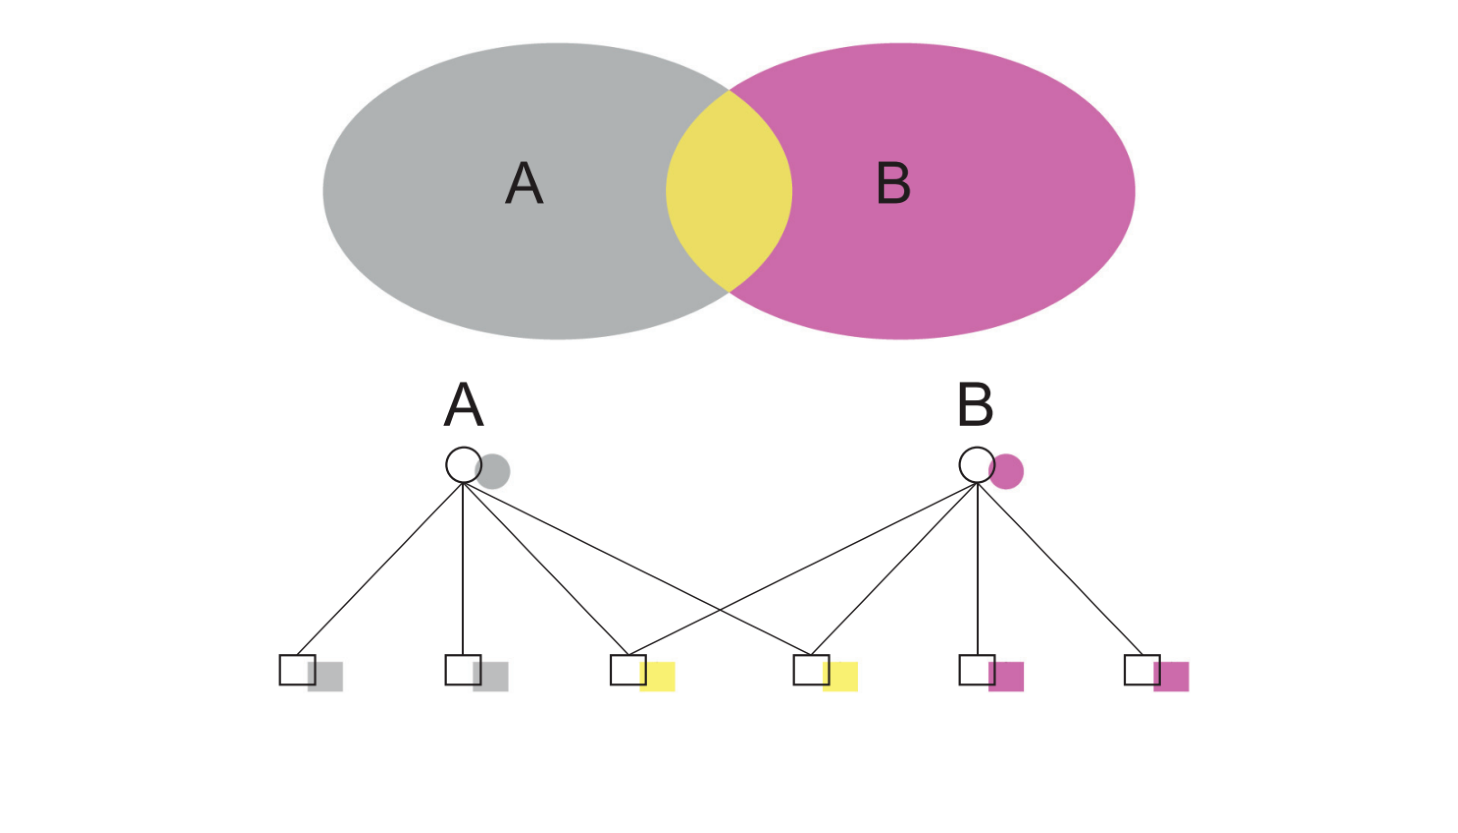
\includegraphics[width=\columnwidth]{img/chapter2/overlapping.pdf} 
	\caption{Overlapping Community Structure where nodes can belong to multiple communities. The figure is contributed from \cite{yang2013overlapping}.}
	\label{fig:c2_overlapping}
\end{figure}  


Overlapping community detection is one of the most fundamental topics and many relevant studies are published. By definition, a node $v$ can belong to multiple communities simultaneously so as to cause the overlaps between communities. Figure \ref{fig:c2_overlapping} visualizes the community structure under overlapping circumstance. The nodes marked in color yellow are affiliated with both community $A$ and $B$. Table \ref{tab:c2_overlapping} categorizes and summarizes the focus of each mentioned study for overlapping community detection.

\begin{table}
	% \scriptsize
	\centering
	%   \vspace{-3em} 
	% \renewcommand{\tabcolsep}{2pt}
	\begin{tabular}{|p{5cm}|p{9cm}|} \hline
		\textbf{References} &  \textbf{Main Idea} \\ \hline
		\cite{coscia2012demon,whang2013overlapping,whang2016overlapping,huang2018overlapping,wang2017overlapping} & Local search and seed expansion\\ \hline
		\cite{yang2013overlapping,zhang2015incorporating,zhang2016modeling,eustace2015overlapping,jin2015combined}& Nonnegative matrix factorization\\ \hline
		\cite{gopalan2013efficient,jin2016detect,}& Bayesian, generative model\\ \hline
		\cite{yang2012community}& Affiliation network\\ \hline
	\end{tabular}
	\caption{The main ideas of mainly introduced overlapping community detection approaches.}
	\label{tab:c2_overlapping}
	
\end{table} 

\cite{amelio2014overlapping} is a survey paper published in 2014. Although the methods introduced within it are sort of dated, it still offers covers several main track methodologies (node seed and local expansion, clique expansion, and label propagation) and particular scenarios (link clustering and dynamic graphs). It draws a conclusion that there is no universal method to deal with all types of graphs with different characteristics in sparsity, degree distribution, and overlap percentage among communities. In the end, it also points out two essential questions to be solved for later researchers, which is ``when to apply overlapping methods and how significant the overlapping is''.  \cite{xie2013overlapping} is another authentic survey paper which reviews a set of methods, benchmarks and evaluation metrics. Besides that, it also reviews papers using stochastic block model or density based models. To study the performance differences among models,  it introduces several benchmark graphs in which node ground truth community is known, i.e. LFR benchmark graph\footnote{https://sites.google.com/site/andrealancichinetti/files}. A set of evaluation metrics including Normalized Mutual Information (NMI) and Omega index are introduced as well. Meanwhile, empirical studies are applied and evaluated on all aforementioned methods using different benchmark graphs. In the end, the paper discovers the sensitivities of different models in sparse graphs appeared in real-world social networks.

DEMON model \cite{coscia2012demon} unveils its overlapping communities with a local-first approach by grouping ego neighbor nodes into the same clusters and finally merges the local communities into a global collection. In the local-first grouping process, DEMON applies a EgoMinusEgo function to first extract ego-based subgraphs for each node $v$ where the node set is node $v$ and all its neighbor nodes $\mathcal{N}(v)$  and the edge set is all graph edges between the selected nodes ($v$ and $\mathcal{N}(v)$). After that, each ego-based subgraph will remove the node $v$ and all its associated edges to achieve an EgoMinusEgo subgraph. An label propagation community detection method is subsequently applied on each EgoMinusEgo subgraph and select a set of largest clusters to best cover the entire graph. In the end, a merging process is applied on the previously generated clusters according to their node similarities and construct the final community partition result. LOSP model \cite{he2015detecting} is another method to explore local neighborhood structures of each node. It defines a Local Spectral Subspace using the first $d$ eigenvectors from the normalized adjacency matrix. In each potential community $c$, a set of seed nodes are given, and an iterative process is applied with the help of seed nodes and the Local Spectral Subspace to rank the top $N_c$ nodes with highest random walk probabilities to appear in the current community. Those nodes are finally regarded as other latent members in each community $c$. 

LOSP model offers a great insight to use seed node expansion to detect overlapped communities. Inspired by LOSP model, \cite{whang2013overlapping,whang2016overlapping} propose a four-phase model including filtering, seeding, seed set expansion, and propagation. The natural of the model first filters out the regions of the graph which don't involve overlapping structure. A seeding strategy inspired by Kmeans selects a set of seed nodes with small Conductance relationship. A seed set expansion approach is further applied by taking advantage of personalized PageRank model to construct raw communities near each seed node. In the last propagation step, the raw communities are expanded again to the regions previously removed in the filtering phase. Similarly, \cite{yang2017finding} also designs a new seeding strategy and expands a set of nodes from seed nodes via a personalized PageRank model. Thereafter it develops a model on the expanded nodes to detect overlapped communities. The seed nodes are the nodes in the maximum spanning tree of the original graph. Personalized PageRank model helps to expand the seed nodes and merge them into raw community structure by maximizing modularity score of the graph. The last optimization step is to merge communities when the shared node ratio of two communities is above an overlapping threshold.

OCD-HSN model \cite{huang2018overlapping} contains a seed selection step as well as community initialization and expansion step to group nodes into clusters in an efficient manner. It claims to be the first research work for overlapping community detection in heterogeneous graph containing both undirected and directed edges. Based on user semantic interests and social connections, this study constructs a heterogeneous graph to hold all types of user profiles. A set of seed nodes are selected based on their centrality and conductance in the graph. The neighbor nodes of the seed nodes naturally  construct overlapped communities. Later on, a fitness evaluation process is leveraged to add or remove nodes  based on the node connectivity in each community. 

Structural centers are defined and utilized in \cite{wang2017overlapping} to support local expansion for overlapping community detection, which are the nodes that have high node degrees and are also far away from other structural centers.


By natural, nonnegative matrix factorization can solve overlapping community detection problem as it can directly learn low dimensional node representation matrix from the graph matrices such as adjacency matrix. Each column in the reduced node represention matrix represents an eigenvector, which also can be regarded as a community. Therefore, the learned node representation can be regarded as the node affiliation distribution over communities. BIGCLAM model \cite{yang2013overlapping} is a classic overlapping community detection model which can take care of large-scale graphs. In its model, $F$ represents a nonnegative matrix where $F_{uc}$ is the affiliation score of node $u \in V$ in community $c \in C$. Given an unlabeled and undirected network $G(V, E)$, BIGCLAM aims to re-generate all graph edges using node's community affiliation distribution. It aims to maximize the probability of node $u$ and $v$ if there is an edge between them and minimize the probability if there is no edge.  Therefore, the objective function $l(F)$ to maximize turns to be:

\begin{equation}
l(F) = \sum_{(u,v) \in E} log(1-exp(-F_uF_v^T)) - \sum_{(u,v) \notin E} F_uF_v^T
\end{equation}

The number of communities can also be determined in the model through an empirical test.
 
PNMF model \cite{zhang2015incorporating} is also a nonnegative matrix factorization model.  Unlike conventional matrix factorization models to directly decompose the original adjacency matrix, PNMF considers the situation that a node prefers its neighbor nodes. Therefore, instead of re-generating the edges between two nodes, this paper considers node triplet $(i,j,k)$.  $j>_{i} k$ denotes that $ j \in \mathcal{N}(i)$ and $k \notin \mathcal{N}(i)$ so that node $i$ prefers $j$ to $k$. And the overall goal of this approach is to maximize this preference likelihood that neighbor nodes should be preferred than non-neighbor nodes:
\begin{equation}
\begin{aligned}
l(F) &= \sum_{(i,j,k) \in S} log(p(j>_{i}k|F) )-\lambda \cdot reg(F) \\
 &=  \sum_{(i,j,k) \in S} log(\sigma(F_iF_j^{T} - F_iF_k^{T}))-\lambda \cdot reg(F)
\end{aligned}
\end{equation}
 where $S$ is pre-sampled node triplet collection which satisfies the node preferences. $reg(F)$ is the regularization term added to avoid overfitting and $\lambda$ is the regularization weight.
 
HNMF \cite{zhang2016modeling} is another nonnegative matrix factorization model which considers both-sided relationships between edges and communities. From the community-to-edge perspective, it takes advantages of PNMF model to maximize the log likelihood of node connection preferences in all sampled node triplets. From the edge-to-community perspective, it uses negative sampling strategy in a skip-gram model to maximize the probability if two nodes are neighbor nodes and minimize the probability if they are not. The final loss is the loss sum from both PNMF and the negative sampling, which is aimed to be maximized in the joint training process. 
 
NRATIO model \cite{eustace2015overlapping} generates a vertex neighborhood ratio matrix to substitute original adjacency matrix or Laplacian matrix. This matrix refines the graph adjacency matrix where two nodes are connected only if their common neighbor nodes surpasses the average number of neighbors in all pairwise nodes. In the next step, nonnegative matrix factorization is applied on the refined matrix to learn a community distribution over each node. As the vertex neighborhood ratio matrix reduces the influence of unrelated nodes in community structures, the number of data points in the matrix are significantly reduced, which fastens the running speed.

\cite{jin2015combined} first describes a stochastic block model to accommodate both node and edge communities, and then uses conductance measurement to fine-tune the learned node community distribution. One outstanding point of this paper is that the model considers edge communities. By definition, in the adjacency matrix $A$, $a_{ij} = 1$ if node $v_i$ and node $v_j$ are connected through an edge. And, in bipartite graph matrix $B$, $b_{ij} = 1$ if node $v_i$ and edge $e_j$ are directly linked each other. The paper aims to learn a node community affiliation matrix $H$ where $h_{ij}$ denotes the propensity of node $v_i$ belonging to community $c_j$ and an edge community affiliation matrix $W$ where $w_{ij}$ denotes the propensity of edge $e_i$ belonging to community $c_j$. In the end, to use the node/edge community information ($W$ and $H$) to re-construct the two matrices $A$ and $B$, the objective function is defined as follows:

\begin{equation} 
	\mathcal{O}(H,W) = ||A-HH^T||^2_F + \lambda ||B-WH^T||^2_F
\end{equation}
where $||\cdot||_F$ is the Frobenius norm, $H$ and $W$ have to be nonnegative matrices.

AGM model \cite{yang2012community} is a preliminary study using affiliation network to re-generate the original social network. Given only the overlapping community affiliation of each node, it learns the  reproduction of original links between nodes in order to construct the social network. The edge generation probability is defined as: 
\begin{equation}
p(u,v) = 1-\prod_{c \in C_{uv}} (1-p_c)
\end{equation}
where $C_{uv}$ are a set of shared communities for node $v$ and $u$. $p_k$ refers to the probability of an edge forming between two nodes in the community $c$. 

\cite{gopalan2013efficient} uses a mixture membership stochastic block model to learn node overlapping communities. The overall framework is a Bayesian approach. It assumes the overlapped community memberships of each node $v_i$ is associated with a Dirichlet distribution $\theta_i$. For each pair of node $v_i$ and $v_j$, it draws a community indicator $z_{i \rightarrow j}$ from node $v_i$’s community membership $\theta_i$ and then draws  a community indicator  $z_{i \leftarrow j}$  from node $v_i$’s community membership $\theta_j$. Each indicator points to one
of the $|C|$ communities. Finally, it draws an edge between two nodes with the generation probability:
\begin{equation} 
p(y_{ij} = 1|z_{i \rightarrow j},z_{i \leftarrow j}) =
\begin{cases}
z_{i \rightarrow j},       & \quad  z_{i \rightarrow j} = z_{i \leftarrow j}\\ 
\epsilon,  & z_{i \rightarrow j} \neq z_{i \leftarrow j}\\ 
\end{cases}
\end{equation}
The whole process is optimized and all nodes' $\theta$ are learned by maximizing the edge generation probability $p(y_{ij} = 1)$from the actual graphs.  $\epsilon$ is a small constant. The
parameter $\beta_{z_{i \rightarrow j}}$ is the density of community $z_{i \rightarrow j}$.

Similarly, \cite{jin2016detect} also introduces a Bayesian based generative model. It assumes a Poisson distribution for node community distribution and is optimized using a Expectation-Maximization (EM) approach. Node communities are selected according to its learned community distribution and related community conductance in the end.

\subsection{Number of Communities}
Among all sorts of community detection models, only few of them can automatically determine the number of communities given the model nature. Most of them need to specify the community number in advance before applying their main processes. Therefore it is still an open question about how to choose the exact community number. Many in-depth researches draw their conclusions either from empirical studies or mathematical proofs. In this section, several works particularly exploring this research question are introduced and discussed, which offers general insights for potential community number selection.

\cite{newman2016estimating} proposes a statistical model using Bayesian inference analysis. It finds the correct number of communities by maximizing the integrated likelihood of graph structure and observed community partition using a generative model. In detail, given the prior knowledge of graph structure (adjacency matrix $A$) and community partition $C$, it uses Markov chain Monte Carlo (MCMC) importance sampling to calculate the posterior distribution of community number $|C|$.

\cite{le2015estimating} develops an efficient model to study community numbers based on graph spectral properties. It statistically proves the number of positive and most informative eigenvalues as the estimated number of communities on five spectral clustering methods which use either the non-backtracking matrix or the Bethe Hessian matrix. 

Moreover, two motivations happened in stochastic block models urge the exploration of community numbers. First, edges are not necessarily independent if only the communities of their endpoint nodes are given. Second, the loss of precision occurred in spectral clustering is inevitable. Therefore, through a set of rigorous proofs, \cite{saldana2017many} proposes a composite likelihood BIC (CL-BIC) model to handle the community number selection  happened in stochastic block model (SBM), degree-corrected block model (DCBM) and mixture-membership block model (MMB). 

For other works relevant to community number selection, \cite{kawamoto2017cross,chen2018network} both leverage the leave-one-out cross-validation to determine the community number by optimizing the edge prediction error and Bethe free energy in stochastic block model.  \cite{kawamoto2018comparative} conducts a comparative analysis on various community detection models (stochastic block model, greedy methods, statistical inference models and spectral methods) to track the changes of assessment criteria (modularity, map equation, Bethe free energy and prediction error and isolated eigenvalues) associated with various of community numbers.

\subsection{Community Search}
Instead of generating communities for all nodes in the graph, community search based approaches aim to find the top relevant subgraphs or communities that match particular purposes, which can be regarded as a mixture of community detection and information retrieval. Currently, there are two main types of search scenarios. One is that given a set of query nodes, return the densest subgraph containing query nodes. The other is given a set of query nodes, return their top $k$ most relevant communities. Relevant works are summarized by main ideas in Table \ref{tab:c2_search}.

\begin{table}
	% \scriptsize
	\centering
	%   \vspace{-3em} 
	% \renewcommand{\tabcolsep}{2pt}
	\begin{tabular}{|p{4.5cm}|p{9.5cm}|} \hline
		\textbf{References} &  \textbf{Main Idea} \\ \hline
		\cite{sozio2010community,cui2014local,barbieri2015efficient,wu2015robust,huang2015approximate} & Return the densest subgraph containing all query nodes\\ \hline
		\cite{chen2012dense,qin2015locally,lancichinetti2011finding,huang2014querying,zheng2017finding,yan2019constrained,li2015influential}& Return top $k$ most relevant/influential communities with or without query nodes \\ \hline 
	\end{tabular}
	\caption{The main ideas of community search approaches.}
	\label{tab:c2_search}
	
\end{table} 


\cite{sozio2010community} is a very classic paper of community search, which is defined as given a graph $G(V,E)$ and a set of query nodes, seeking a a subgraph of $G$ which contains all the query nodes and meanwhile is densely connected. The nodes with trivial degrees and far away from query nodes are filtered out from the community. The final goal of this paper is to maximize the minimum degree of a subgraph containing all query nodes. A greedy solution is proposed by deleting each node with minimum degree at each step. The iterative process terminates either at least one of the query node reaches to the minimum degree or is no longer connected with the rest of nodes. Further two heuristic approaches are extended to detect the community with an upper bound size restriction. 

\cite{cui2014local} is a subsequent work of the previous one, which aims to detect the best community for a given node. It formulates and solves two community search problems: communitysearch with a threshold constraint (CST) problem and community search with a maximality constraint (CSM) problem. Two approaches including global search and local search are proposed where the second approach is more efficient than the first one because of reducing searching space significantly.  

\cite{barbieri2015efficient} is another follow-up work of \cite{sozio2010community}. It improves the model efficiency and accuracy as one limitation of the previous work  is that it tends to find quite large solutions, which negatively affects the detected community accuracy. Unlike the \cite{sozio2010community} in which the community size is constrained, it aims to detect the smallest-size community among all optimal ones. In detail, it computes the core decomposition and organizes the retrieved k-cores (maximal subgraphs where each nodes are connected at least $k$ other nodes in a subgraph). In the end, a greedy-connection approach is leveraged to use a local search method to reduce the potential subgraph size (greedy step) and a Steiner Tree-based strategy to find the minimum number of nodes that make all query nodes connected.
 
Given a query node, \cite{wu2015robust} formulates a query biased densest connected subgraph (QDC) problem which aims to find the densest subgraphs that contains the query nodes and is also internally connected. A densest subgraph can be regarded as a local community in this paper. To reduce a free rider effect which involves irrelevant nodes into densest subgraphs, a random walk based weighting scheme is proposed to set higher penalties to these irrelevant nodes when they are included in the subgraphs/communities. 

\cite{huang2015approximate} solves a closest truss community (CTC) problem which finds a connected k-truss subgraph with the largest $k$ and minimum graph diameter.  By its definition, a k-truss subgraph requires each edge is contained in at least $k-2$ triangles  in the subgraph. A greedy algorithm is proposed to first find a raw CTC that contains all query nodes, then iteratively removes the furthest nodes in the CTC to finally achieve the optimized subgraph.
 
\cite{chen2012dense} introduces a partial clustering model to extract the most dense subgraphs, meanwhile it does not require to determine the number of subgraphs in advance. The model is inspired by the matrix blocking problem to reorder the adjacency matrix $A$ and to find the dense diagonal blocks as extracted subgraphs. It considers three types of graph scenarios including undirected graph, directed graph and bipartite graph. By calculating the pairwise columns in the adjacency matrix, it obtains the similarities between all pairs of nodes, which is stored as matrix $M$. The final goal turns to reorder the rows and columns of $M$ so that inside each nontrivial diagonal block of matrix $M$, there exists at least one datapoint larger than a threshold for each row and column. It means that for each node in the diagonal block, there exists at least one other node densely connected with it. To accelerate the running speed, a hierarchical optimization approach is proposed in a top-down manner. The large generated diagonal blocks are finally regarded as extracted dense graphs. 

 \cite{qin2015locally} aims to retrieve top $k$ locally densest subgraphs (LDS) which are particularly defined in the paper. LDS is defined based on density (nodes within the LDS are densely connected) and compactness (removing a node in LDS will lose significant number of edges within it). With solid proofs, LDS  should satisfy a set of structural properties in compactness, cohesive and disjoint property. The original optimization approach is based on greedy algorithm, which runs in polynomial time. To reduce this running time, three optimization strategies are applied including pruning invalid nodes, optimization in finding dense subgraphs and optimization in verifying whether the dense graphs are eligible LDS.
 
OSLOM model \cite{lancichinetti2011finding} finds statistically significant communities through local optimization of a fitness function (significance score) which considers single cluster analysis and full network analysis. In single cluster analysis, the significance of a community is defined as the probability of finding the community in a random null model. In full network analysis, an iterative approach is leveraged to optimize the whole graph-level significance score by grouping nodes into proper communities. The approach first adds external nodes to existing subgraphs based on the generative probability. After that non-significant nodes are removed from the updated subgraphs.  

\cite{huang2014querying} regards a node as a query in the graph, and retrieves its k-truss communities through a designed compact and elegant index structure, which makes the overall model scalable with linear cost to serve online community search tasks.  On top of k-truss subgraph, k-truss community is defined with an extra edge connectivity constraint to ensure its node connectivity, which is any two edges in a k-truss community should either belong to the same triangle, or are reachable from each other through a series of adjacent triangles. To accelerate the running speed, a simple k-truss index are developed using an existing truss composition algorithm. Further an enhanced TCP-index is proposed to avoid two drawbacks from previous index: unnecessary access of dis-qualified edges and repeated access of qualified edges. 

Having the same research goal, \cite{zheng2017finding} takes edge weights into account to support better k-truss community detection for query nodes. It firstly utilizes a Breadth first search (BFS) method by removing unimportant edges iteratively. However this BFS approach suffers high computational cost which can not deal with large scale graph. To tackle this problem, it designs a KEP-index (Key Edges Preserved Index) which stores all possible k-truss community candidates in a space-efficient index structure. In the index construction process, communities are decomposed (edges are removed) in a hierarchical manner and the related key edges to reconstruct the hierarchical community tree are stored in the tree-shaped index. 

\cite{yan2019constrained} takes advantages of random walks to detect local graph communities. Starting from a set of seed nodes with given community memberships, the method labels each seed nodes with same/different colors according to its community. And a color-based random walk is applied to propagate colors across nodes to detect all other nodes communities. To store the color of each node, $K$ transition matrices are maintained where $K$ refers to the number of distinct colors in the seed nodes. Throughout an iterative propagation process, the color of each node can be learned and updated by its last-iteration color and the propagated colors from its neighbor nodes. The final color of the nodes are their deterministic community labels. 

Derived from k-core, \cite{li2015influential} proposes an online search algorithm to find the top k-influential communities in linear time through a linear-space index structure. A k-influential community means each node weight within should be at least $k$. The paper introduces a basic algorithm, a depth first search (DFS) and a final index based algorithm. The index based algorithm is able to handle large networks and runs in linear time. It uses a tree/forest index structure to hold all k-influential communities and utilizes a DFS function to iteratively add/remove nodes for index organization until all possible communities are scanned. 

\subsection{Community Detection Enhancement}

Enhancing community detection performance is also an essential task as it provides extra in-depths supports to explore how to improve model performance. As there is no main trend in this research topic, different types of approaches are introduced here with dispersive solutions, including assigning edge weights, removing unimportant nodes, or involving external information, etc. 

\cite{khadivi2011network} assigns proper edges weights on unweighted graphs to circumvent resolution limit \& extreme degeneracy problems and in the end enhances the performance of modularity based methods. modularity has been proved to suffer a resolution limit problem that the community size is constrained. With solid proofs, applying a weighted modularity can increase the upper bound and decrease the lower bound of community size. It allows to detect both larger and smaller communities using weighted modularity methods. Extreme degeneracy problem means that it goes more and more difficult to find the optimal community partition when the community size is large. And a proper weighting schema is able to strength the intra-community edges and weaken the rest to better clarify the community boundary. The weighting schema is defined as:

\begin{equation}
	W_{ij} = 
	\begin{cases}
	\frac{b_{ij}^{-\alpha}\cdot C_{ij}^{\beta}}{\sum_{k,m;k\neq m}b_{km}^{-\alpha}\cdot C_{km}^{\beta}},       & A_{ij} = 1\\ 
	0,  & A_{ij} = 0\\ 
	\end{cases}
\end{equation}
where $\alpha$, $\beta$ are positive numbers, $b_{ij}$ is the edge betweenness score and $C_{ij}$ is the common neighbor ratio between node $v_{i}$ and $v_j$.  \cite{de2013enhancing} proposes a similar weighting strategy that edges are weighted according to their betweeness centrality score. The proposed WERW-Kpath approximately estimates edge betweenness  score as the traversed probability of $\rho$ random walks with at most $k$ steps started from random nodes. This approximation reduces the NP hard edge weighting problem to a situation with worst time complexity as $\mathcal{O}(k|E|)$.

\cite{lai2010enhanced} shows a network preprocessing step can helps to alleviate the resolution limit problem for modularity based algorithms. It assigns random walks on graphs. By tracking these random walk trajectories, the similarity score of each pair of nodes are calculated as the updated weights in the original graph. The iterative steps run for several rounds and the modularity based community detection is applied in the last phase of graph.

\cite{wen2011improving} raises a point that hub nodes which are connected with many other nodes can disturb the community structure. Therefore, it proposes a degree-targeted node removal approach to reduce such noise. In detail,  it exhaustively searches through each node and introduces two types of approaches. First, the nodes with highest degrees are regarded as noisy nodes to remove. Second, the nodes whose removal causes the largest increase in modularity are regarded as noisy nodes to remove. 

\cite{he2016model} first calculates the structural similarity of each pair of nodes based on their degrees. A strong constraint matrix and a weak constraint matrix are both derived from node pairwise similarities. Further on, these matrices are incorporated into a stochastic block model to enhance the community detection. Intuitively, it aims to group each node in the same community with its high-similarity nodes and separate with low-similarity nodes in different communities. The parameters to be learned are optimized through a nonnegative matrix factorization approach. 

\cite{zhang2013enhanced} designs a semi-supervised algorithm to incorporate prior knowledge to guide the detection process. The prior knowledge utilized in the study contains must-link and cannot-link. It simply applies this information in the adjacency matrix $A$: If node $v_i$ and $v_j$ have a must-link, the weight of $e_{ij} = \alpha$; If node $v_i$ and $v_j$ have a cannot-link, the weight of $e_{ij} = 0$. It further extends to another refined adjacency matrix but involving a third node $v_k$: If $v_i$ and $v_j$ have a must-link and $v_i$ and $v_k$ have a must-link, then $v_j$ and $v_k$ should also have a must-link (the friend of my friend is my friend); If $v_i$ and $v_j$ have a must-link and $v_i$ and $v_k$ have a cannot-link, then $v_j$ and $v_k$ should also have a cannot-link (the friend of my enemy is my enemy). Conventional community detection methods can be directly applied on the refined adjacency matrix to get the enhanced community partition.

\cite{zhou2019adversarial} is the latest work which introduces two adversarial enhancement methods for community detection. One is called AE-GA, which is a genetic based adversarial algorithm to determine optimal edge modification and rewire community connections. Each chromosome in the genetic algorithm is a set of edges to be added or deleted in the graph. The fitness function is a variant of modularity:

\begin{equation}
f = \frac{\mathcal{Q}}{e^{|M_S - M_{real}|}}
\end{equation}  

where $\mathcal{Q}$ is current partition's modularity score. $M_{real}$ is the number of the ground-truth communities in graph $G$. $M_S$ is the number of communities detected by an particular method $S$. Another proposed model is called AE-VS model, which enhance the graph structure using node similarities. In detail, it rewires a graph by adding/deleting edges with a consideration of multiple similarity metrics and aggregates scattered communities to a better core community.

EdMot model \cite{li2019edmot} is a Motif-aware community detection. A motif-based hypergraph is constructed from the original graph to encode higher order node connections. Each of the top $K$ largest connected components, with the most number of nodes, is individually partitioned into communities through modularity-based methods. All the potential edges (generated from each pair of nodes) within each community are strengthened to put back to the original graph for enhanced community detection. 

\cite{veldt2019learning} presents a way to automatically learn the resolution parameters in community detection to control the size of communities. It is formulated to optimize a parameter fitness function which generally measures how these parameters can solve a generalized community question through a set of solid proofs. \cite{bhatt2019knowledge} incorporates hierarchical concepts of node attributes  into community detection. It detects node communities and simultaneously maintains the coherence of community label/context  summarized from node attributes. 

\subsection{Semi-Supervised Community Detection}
Conventional community detection approaches should be unsupervised and only leverage graph topological structures. However, unsupervised approaches are always weak in terms of model performance due to no-label guidance in the learning process. Therefore, to improve the model performance, partial information/constraints (must-links and cannot-links) are obtained to guide the learning process to the right direction, which forms the semi-supervised community detection task. 

SNMF-SS model \cite{ma2010semi} combines symmetric nonnegative matrix factorization and a semi-supervised approach where domain knowledge is incorporated to guide the detected communities. It provides two type of domain knowledge including must-links ($W_{ML}$) and cannot-links ($W_{CL}$). Each datapoint $w_{ij} \in W_{ML}$ means the edge between node $v_i$ and $v_j$ is given, and $w_{ij} \in W_{CL}$ means there should not be an edge between the two nodes. In the end, the paper aims to learn a low dimensional representation of nodes by optimizing the following objective function:

\begin{equation}
\argmin_{\hat{A} \geq 0, H \geq 0} || \hat{A} - HH^{T} ||^2
\end{equation}

where $\hat{A} = A - \alpha W_{ML} + \beta W_{CL}$ and $A$ is the adjacency matrix. $H$ is the low dimensional node matrix to be learned. 
 
SSNMF model \cite{liu2017semi} involves must-links $M$ as prior information into a nonnegative matrix factorization framework to alleviate the negative impacts from node degree heterogeneity.  In this model, two nodes having a must-link should be restrictively grouped into the same community using the learned low dimensional node representation matrix from NMF approach. It turns to minimize the representation difference between the two nodes having must-links. And the final objective function to minimize turns to be the weighted sum of must-link restrictions and original NMF objective function:
\begin{equation}
  \argmin_{\hat{A} \geq 0, H \geq 0} || \hat{A} - HH^{T} ||^2 + \lambda \sum_{ij}||h_i - h_j|| M_{ij}
\end{equation}
where $H$ is the low dimensional node representation matrix and $h_{i} \in H$ refers to the node $v_{i}$'s representation. 

PCSEO-SS model \cite{li2014extremal} is able to detect false connections and conflicted connections. In detail, it utilizes a dissimilarity index metric which describes the probability of two nodes belong to the same community. Higher value refers to less same-community probability. Prior node pairwise constraints (must-links and cannot-links) are corrected by setting up a threshold on the dissimilarity index.  Then an approach is given to maximize the modularity of the graph by removing extra-community edges iterative and in the end constructs the final community partition. 

\cite{cheng2014active} also makes full use of node pairwise constraints including must-links and cannot-links to extract high-quality communities. First, The two nodes in each cannot-link are forced to be grouped into different communities, which forms the skeleton of the overall community structure. Second, the communities containing nodes involved in must-links are merged into the same community without violating the existing skeleton community structure. After the nodes in must-links and cannot-links are processed, a greedy algorithm is applied to classify each of the remaining nodes into the existing raw communities. The nodes are selected and assigned to communities based on its similarity between each community and itself. 

\cite{yang2015active} proposes an iterative approach containing three steps. First, it applies nonnegative matrix factorization on the adjacency matrix to obtain the community structure. Second, for some pairs of nodes, their edges are uncertain but informative. The model designs a Connection Strategy by using human labeling on these edges to identify whether these edges should exist or not. Third, for these labeled new edges, a Disconnection Strategy is applied to highlight their importance weight, leading a result of  graph topological reconstruction. The three steps are optimized iteratively and the final round result will be regarded as the final community partition.

 \cite{jin2019graph} is the latest work by combining deep learning, Graph Convolutional Network (GCN), and statistical model, Markov Random Fields (MRF) to solve attribute graph community detection. The introduced end-to-end approach contains three layers. The first two layers are GCN layers which utilized both adjacency matrix $A$ and attribute matrix $X$ to learn the node community labels. The third layer is a MRF layer to refine the community partition result by enhancing node pairwise potential relationships. 
 
 WSCDSM model \cite{wang2018unified} contains two parts: A nonnegative matrix factorization approach with prior must-links to detect node communities and a semantic driven community detection via node content information. In the end, it integrates the two parts of the model into a unified framework and detects both topological and semantic communities. The training process combines the two individual objective functions together and uses a stochastic gradient descent method to optimize the two communities of each node.
 
 For other types of approaches, \cite{eaton2012spin} uses spin-glass model,  \cite{zhang2014phase} studies belief propagation and the stochastic block model, and \cite{yang2014unified} adds graph regularizations to penalize the dissimilarities between node pairs which should be in the same communities. 
 
\subsection{Summary}

I  formulate five different community detection tasks and introduce the best representative works of each task in the recent decade to demonstrate an overview. In fact, for each task, more and more research works having been published each year as the graph mining domain is with an increasing trend. Among the five tasks, overlapping community detection is the largest track which attracts the most researchers' attention for years. A rich number of papers are published regarding as this topic to the venues in computer science and physics domain. Semi-supervised approaches are also popular these years because empirical studies show that unsupervised learning approaches performs far worse than supervised ones. Moreover, beyond these five tasks, there are also many other tasks which focus on other perspectives towards community detection, such as Motif-based problems, math proofs, and edge community detection. In the future, more other interesting topics will be proposed, explored, and summarized. 